\chapter{Theoretical Proofs and Derivations}\label{sec:appendix_theory}

We will define some notation shortcuts for the following proofs.

\section{Proof of problem formulation}\label{sec:proofs}

\begin{lemma} 
    
    Let $N, K \in \mathbb{N}$ and let $\left\{\mathcal{E}_{i j} \mid i \leq N, j \leq K\right\}$ be an indexed set of values. Then,
    $$
    \sum_{c \in \mathcal{C}} \prod_{i=1}^N \mathcal{E}_{i, c(i)}=\prod_{i=1}^N \sum_{j=1}^K \mathcal{E}_{i j}
    $$
\end{lemma}

\begin{proof}
By induction on $N$. For the $N=1$ base case, observe that $\mathcal{C}$ has only $K$ elements, as there are only $K$ functions mapping $\{1\}$ to $\{1, \ldots, K\}$. Then
$$
\sum_{c \in \mathcal{C}} \prod_{i \leq N} \mathcal{E}_{i, c(i)}=\sum_{c \in \mathcal{C}} \mathcal{E}_{1, c(1)}=\sum_{j \leq K} \mathcal{E}_{1, j}=\prod_{i \leq N} \sum_{j \leq K} \mathcal{E}_{i, j} .
$$

Assume now that the result holds for some $N$. We demonstrate then that it also holds for $N+1$. Observe that there is a bijection between $\mathcal{C}$ and $\{1, \ldots, K\}^N$. Therefore, we identify every function $c \in \mathcal{C}$ with the tuple $(c(1), \ldots, c(N))$. Conversely, we identify every tuple $\left(c_1, \ldots, c_N\right) \in\{1, \ldots, K\}^N$, with the function $c$ that maps $i$ to $c_i$.

$$
\begin{aligned}
    & \sum_{c \in \mathcal{C}} \prod_{i \leq N+1} \mathcal{E}_{i, c(i)}= \\
    & =\sum_{\left(c_1, \ldots, c_{N+1}\right) \in\{1, \ldots, K\}^{N+1}} \prod_{i \leq N+1} \mathcal{E}_{i, c_i} \\
    & =\sum_{\substack{\left(c_1, \ldots, c_N\right) \in\{1, \ldots, K\}^N \\
    c_{N+1} \leq K}} \prod_{i \leq N+1} \mathcal{E}_{i, c_i} \\
    & =\sum_{\left(c_1, \ldots, c_N\right) \in\{1, \ldots, K\}^N} \sum_{c_{N+1} \leq K} \prod_{i \leq N+1} \mathcal{E}_{i, c_i} \\
    & =\sum_{\left(c_1, \ldots, c_N\right) \in\{1, \ldots, K\}^N} \sum_{c_{N+1} \leq K}\left(\mathcal{E}_{N+1, c(N+1)} \prod_{i \leq N} \mathcal{E}_{i, c_i}\right) \\
    & =\left(\sum_{c_{N+1} \leq K} \mathcal{E}_{N+1, c(N+1)}\right) \sum_{\left(c_1, \ldots, c_N\right) \in\{1, \ldots, K\}^N} \prod_{i \leq N} \mathcal{E}_{i, c_i} \\
    & =\left(\sum_{c_{N+1} \leq K} \mathcal{E}_{N+1, c(N+1)}\right) \prod_{i \leq N} \sum_{j \leq K} \mathcal{E}_{i, j} \\
    & =\left(\sum_{j \leq K} \mathcal{E}_{N+1, j}\right) \prod_{i \leq N} \sum_{j \leq K} \mathcal{E}_{i, j} \\
    & =\prod_{i \leq N+1} \sum_{j \leq K} \mathcal{E}_{i, j} . \\
    &
    \end{aligned}
$$
\end{proof}


\begin{theorem}[Posterior factorization]

    The posterior distribution for a classification problem can be factorized as follows:
    $$
    \mathbf{P}^c(\theta \mid \bm{x}) = \prod_i^N  \mathbf{P}^c(\theta_i \mid \bm{x}) = \prod_{i=1}^N \frac{\exp \left ( \beta F_{\theta_i}(x_i) \right )}{\sum_{j=1}^K \exp \left ( \beta F_j(x_i) \right )}
    $$
\end{theorem}

\begin{proof}
    The posterior distribution solution to the MAP problem is the following:

    $$
    \mathbf{P}^c(\theta \mid \bm{x}) \frac{\exp \left ( \beta \sum_{i=1}^N F_{\theta_i}(x_i) \right )}{\sum_{\theta \in \Theta} \exp \left ( \beta \sum_{i=1}^N F_{\theta_i}(x_i) \right )}
    = \frac{\prod_{i=1}^N \exp \left ( \beta F_{\theta_i}(x_i) \right )}{\sum_{\theta \in \Theta} \prod_{i=1}^N \exp \left ( \beta  F_{\theta_i}(x_i) \right )}
    $$

    Using Lemma \ref{lemma:exchangeability} we can rewrite the denominator as:

    $$
    \sum_{\theta \in \Theta} \prod_{i=1}^N \exp \left ( \beta  F_{\theta_i}(x_i) \right ) = \prod_{i=1}^N \sum_{\theta \in \Theta} \exp \left ( \beta  F_{\theta_i}(x_i) \right )
    $$

    Therefore, the posterior distribution can be written as:

    $$
    \mathbf{P}^c(\theta \mid \bm{x}) = \prod_{i=1}^N  \mathbf{P}^c(\theta_i \mid \bm{x}) = \prod_{i=1}^N \frac{\exp \left ( \beta F_{\theta_i}(x_i) \right )}{\sum_{\theta \in \Theta} \exp \left ( \beta R(\theta, \bm{x}) \right )}
    $$

\end{proof}

\section{Properties of the PA kernel}\label{sec:appendix_pa}

\begin{theorem}[Symmetry of the PA kernel]
    The posterior agreement kernel is symmetric with respect to the definition of $X'$ and $X''$.

    $$
    PA(\bm{x}', \bm{x}'') = PA(\bm{x}'', \bm{x}')
    $$
\end{theorem}

\begin{proof}
    Trivial, commutative property.
\end{proof}

\begin{theorem}[Non-negativity of the PA kernel]
    The posterior agreement kernel is non-negative.

    $$
    PA(\bm{x}', \bm{x}'') \geq 0
    $$  
\end{theorem}

\begin{proof}
    See Lemma \ref{lemma:pa}.
\end{proof}

\begin{theorem}[Concavity of the PA kernel]
    The posterior agreement kernel is concave in $\mathbb{R}^+$, and therefore
    has a unique maximum.
\end{theorem}

\begin{proof}

The posterior agreement kernel has been shown to have the following form:

$$
\operatorname{PA}\left(\bm{x}', \bm{x}'' \right) \propto \sum_{n=1}^N \log \left[ \sum_{j=1}^K \mathbf{P}_n^c(\theta \mid x_n') \mathbf{P}_n^c(\theta \mid x_n'') \right]
$$

where the posteriors $\mathbf{P}_n^c(\theta \mid x_n)$ are Gibbs distributions for each observation.

$$
\mathbf{P}_n^c(\theta \mid x_n') = \frac{e^{\beta F_j(x_n)}}{\sum_{k=1}^K e^{\beta F_k(x_n)}}
$$

We will require three important results from optimization theory:

\begin{description}
    \item[T1] The minimum of $G(\beta) = -\operatorname{PA}(X', X'')$ over the convex set $\mathbb{R}^+$ is unique $\iff$ $G(\beta)$ is convex.
    \item[T2] $G$ is absolutely convex $\iff$ $\frac{d^2}{d \beta^2} G(\beta) > 0$.
    \item[T3] The sum of convex functions is also convex.
\end{description}


To streamline the derivation, the following notation will be used:

$$
F_j(x_n') = F'_j
$$

$$
e^{\beta F_j(x_n')} = e^{\beta F'_j} = e'_j
$$

The observation index $n$ will be omitted as it does not affect the convexity derivation (see \textbf{T3}). With that notation in mind, we can define $G(\beta)$ properly:

$$
G(\beta) = -k(\bm{x}', \bm{x}'') = \sum_{n=1}^N - \log \left [\sum_{j=1}^K e'_j e''_j \right] + \sum_{n=1}^N \log \left [ \sum_{k=1}^K e'_k \sum_{p=1}^K e''_p \right] 
$$

We will focus on the first term: $G^n_1(\beta) = G_1(\beta) = \log \left [\sum_{j=1}^K e'_j e''_j \right]$.

$$
\frac{d}{d \beta} G_1(\beta) = \frac{\sum_{j=1}^K (F'_j + F''_j)e'_j e''_j }{\sum_{j=1}^K e'_j e''_j }
$$

We will recurrently use the derivative $\frac{d}{d \beta} e'_j e''_k$ in this proof:

$$
\frac{d}{d \beta} e'_j e''_k = F'_j e'_j e''_k +e'_j F''_k  e''_k = (F'_j + F''_k) e'_j e''_k
$$

The second derivative is straightforward:

$$
\frac{d^2}{d \beta ^2} G_1(\beta) = \frac{\sum_{j=1}^K (F'_j + F''_j)^2 e'_j e''_j }{\sum_{j=1}^K e'_j e''_j } - \frac{\left (\sum_{j=1}^K (F'_j + F''_j) e'_j e''_j \right ) ^2}{\left (\sum_{j=1}^K e'_j e''_j \right )^2}
$$

We impose the convexity condition and see whether it can be contradicted.

$$
\frac{d^2}{d \beta ^2} G_1(\beta) > 0 \iff \left(\sum_{j=1}^K e'_j e''_j \right ) \left( \sum_{j=1}^K (F'_j + F''_j)^2 e'_j e''_j  \right ) - \left (\sum_{j=1}^K (F'_j + F''_j) e'_j e''_j \right )^2 > 0
$$

Using the distributive property of the product over the sum, we can reindex our expression:

$$
\sum_{k=1}^K \sum_{j=1}^K (F'_j + F''_j)^2 e'_j e''_j e'_k e''_k - \sum_{k=1}^K \sum_{j=1}^K (F'_j + F''_j) (F'_k + F''_k) e'_j e''_j e'_k e''_k > 0 \iff
$$

$$
\iff \sum_{k=1}^K \sum_{j=1}^K [(F'_j + F''_j) - (F'_k + F''_k) ] (F'_j + F''_j) e'_j e''_j e'_k e''_k  > 0
$$

As we can see, $\Delta_{(jj), (kk)} $ corresponds to the difference in the cost attributed to reference class $j$ and the cost attributed to class $k$, accumulated over $\bm{x}', \bm{x}''$. We can intuitively devise some symmetry in these terms, and we formalize it as follows:

$$
E_{jk} = e'_j e''_j e'_k e''_k = E_{kj}
$$

$$
\Delta_{(jj), (kk)} = (F'_j + F''_j) - (F'_k + F''_k) = (F'_j - F'_k) + (F''_j - F''_k) = - \Delta_{(kk), (jj)}
$$

 Even if $\Delta_{(jj), (jj)} = 0$, we will still include this term to facilitate with the indexing. Overall, the sum can be expressed as:

$$
 \sum_{k=1}^K \sum_{j=1}^K [(F'_j + F''_j) - (F'_k + F''_k) ] (F'_j + F''_j) e'_j e''_j e'_k e''_k = \sum_{k=1}^K \sum_{j=1}^K (F'_j + F''_j) E_{jk} \Delta_{(jj), (kk)} = \sum_{k=1}^K \sum_{j=1}^K S_{(jj), (kk)}
$$


Then, the pairwise sum of symmetric combinations of indexes $k$ and $j$ yields

$$
\begin{aligned}
    S_{(jj), (kk)} + S_{(kk), (jj)} & = (F'_j + F''_j) E_{jk} \Delta_{(jj), (kk)} + (F'_k + F''_k) E_{kj} \Delta_{(kk), (jj)} \\
    & = E_{jk}\Delta_{(jj), (kk)} [(F'_j + F''_j) - (F'_k + F''_k)] = E_{jk}\Delta_{(jj), (kk)}^2 > 0
\end{aligned}
$$


Given that the indexing sets in our nested sum are the same, it's straightforward to see that all the terms will be strictly positive, and the overall sum will be zero only if $e_j = 0 \; \forall j=\{ 1,...K \}$, which is not possible in a classification setting since $\beta \in \mathbb{R}^+$. We end up with the following expression:

$$
\frac{d^2}{d \beta ^2} G_1(\beta) = \sum_{k=1}^K \sum_{j<k}^K E_{jk}\Delta_{(jj), (kk)}^2 > 0
$$

Now we proceed analogously with the second term: 

$$
G^n_2(\beta) = G_2(\beta) = \log \left [\sum_{j=1}^K e'_j \sum_{k=1}^K e''_k \right] = \log \left [\sum_{k=1}^K \sum_{j=1}^K e'_j e''_k \right]
$$

$$
\frac{d}{d \beta} G_2(\beta) = \frac{\sum_{k=1}^K \sum_{j=1}^K (F'_j + F''_k) e'_j e''_k}{\sum_{k=1}^K \sum_{j=1}^K e'_j e''_k}
$$

$$
\frac{d^2}{d^2 \beta} G_2(\beta) = \frac{\sum_{k=1}^K \sum_{j=1}^K (F'_j + F''_k)^2 e'_j e''_k}{\sum_{k=1}^K \sum_{j=1}^K e'_j e''_k} - \frac{\left(\sum_{k=1}^K \sum_{j=1}^K (F'_j + F''_k) e'_j e''_k \right)^2}{\left( \sum_{k=1}^K \sum_{j=1}^K e'_j e''_k\right)^2} > 0 \iff
$$
$$
\iff \left(\sum_{k=1}^K \sum_{j=1}^K e'_j e''_k \right) \left(\sum_{k=1}^K \sum_{j=1}^K (F'_j + F''_k)^2 e'_j e''_k \right) - \left(\sum_{k=1}^K \sum_{j=1}^K (F'_j + F''_k) e'_j e''_k \right)^2 > 0 \iff
$$
$$
\iff \sum_{k=1}^K \sum_{q=1}^K \sum_{j=1}^K \sum_{i=1}^K (F'_j + F''_k)^2 e'_j e''_k e'_i e''_q - (F'_j + F''_k) e'_j e''_k (F'_i + F''_q) e'_i e''_q > 0 \iff
$$
$$
\iff \sum_{k=1}^K \sum_{q=1}^K \sum_{j=1}^K \sum_{i=1}^K (F'_j + F''_k) e'_j e''_k e'_i e''_q [(F'_j + F''_k) - (F'_i + F''_q)] > 0
$$

We can define as well:

$$
\frac{d^2}{d^2 \beta} G_2(\beta) = \sum_{k=1}^K \sum_{q=1}^K \sum_{j=1}^K \sum_{i=1}^K S_{(jk),(iq)} = \sum_{k=1}^K \sum_{q=1}^K \sum_{j=1}^K \sum_{i=1}^K (F'_j + F''_k) E_{(jk),(iq)} \Delta_{(jk),(iq)} 
$$

$$
E_{(jk),(iq)} = e'_j e''_k e'_i e''_q = E_{(ik),(jq)} = E_{(jq),(ik)} = E_{(iq),(jk)}
$$

$$
\Delta_{(jk),(iq)} = (F'_j - F'_i) + (F''_k - F''_q) = - \Delta_{(iq),(jk)}
$$

The symmetry arises when adding two elements that have mirror indexes in both $\bm{x}'$ and $\bm{x}''$.

$$
\begin{aligned}
S_{(jk),(iq)} + S_{(iq),(jk)} & = (F'_j + F''_k) E_{(jk),(iq)} \Delta_{(jk),(iq)} + (F'_i + F''_q) E_{(iq),(jk)} \Delta_{(iq),(jk)} \\
& = E_{(jk),(iq)} \Delta_{(jk),(iq)} [(F'_j + F''_k) - (F'_i + F''_q)] = E_{(jk),(iq)} \Delta_{(jk),(iq)}^2 > 0
\end{aligned}
$$

Given that symmetries are independent for $\bm{x}'$ and $\bm{x}''$, we end up with a similar expression:

$$
\frac{d^2}{d \beta ^2} G_2(\beta) = \sum_{k=1}^K \sum_{q<k}^K \sum_{j=1}^K \sum_{i<j}^K E_{(jk),(iq)}\Delta_{(jk),(iq)}^2 > 0
$$

Even if a further simplified version can be obtained, this one will allow us to complete the proof. We can now define the function $G(\beta)$ as the sum of the two terms:

$$
\frac{d^2}{d \beta ^2} G(\beta) = \sum_{n=1}^N \left [ \sum_{k=1}^K \sum_{q<k}^K \sum_{j=1}^K \sum_{i<j}^K E_{(jk),(iq)}\Delta_{(jk),(iq)}^2 - \sum_{k=1}^K \sum_{q<k}^K E_{(qq), (kk)}\Delta_{(qq), (kk)}^2 \right ]
$$

where we can clearly see that the particular case $\{ k=j, q=i \}$ cancels the negative terms:

$$
\begin{aligned}
    \frac{d^2}{d \beta ^2} F^n(\beta) & = \sum_{k=1}^K \sum_{q<k}^K \sum_{j = \{ 1:K \} \setminus \{ k \} } \sum_{i = \{ 1:K | i < j\} \setminus \{ k \} } E_{(jk),(iq)}\Delta_{(jk),(iq)}^2  \\ 
    & + \sum_{k=1}^K \sum_{q<k}^K E_{(qq), (kk)}\Delta_{(qq), (kk)}^2 - \sum_{k=1}^K \sum_{q<k}^K E_{(qq), (kk)}\Delta_{(qq), (kk)}^2 = \\
    & = \sum_{k=1}^K \sum_{q<k}^K \sum_{j = \{ 1:K \} \setminus \{ k \} } \sum_{i = \{ 1:K | i < j\} \setminus \{ k \} } E_{(jk),(iq)}\Delta_{(jk),(iq)}^2 > 0
\end{aligned}
$$

Which proves that $G(\beta)$ is absolutely convex in $\mathbb{R}^+$:

$$
 \frac{d^2}{d \beta ^2} G(\beta) = \sum_{n=1}^N \frac{d^2}{d \beta ^2} G^n(\beta) = \sum_{n=1}^N \left[ \sum_{k=1}^K \sum_{q<k}^K \sum_{j = \{ 1:K \} \setminus \{ k \} } \sum_{i = \{ 1:K | i < j\} \setminus \{ k \} } E_{(jk),(iq)}\Delta_{(jk),(iq)}^2 \right] > 0
$$

We must note that on the limit $\beta \to \infty$ the curvature is not defined, so it will be always a good practice to start the numerical procedure at a value $\beta_0 = 0^+$:

$$
\lim_{\beta \to 0^+} \frac{d^2}{d \beta ^2} G(\beta) > 0
$$

\end{proof}


\begin{properties}
    $\operatorname{PA}\left(\bm{x}', \bm{x}'' ; \beta\right)$ has the expected behaviour in
    the artificial classifier examples.
    
    \begin{description}
        \item[C1] In a random classifier, accuracy tends to 50\% as sample size grows, but the posteriors 
        are not necessarily paired. The highest agreement will be achieved when posteriors are
        completely flat; that is, when $\beta = 0$. In general:
    
        $$
        \operatorname{PA}\left(\bm{x}', \bm{x}'' ; \beta \right) \leq N \log \frac{1}{2} \;\;\; \forall \beta \in \mathbb{R}^+, \;\; \text{with } \lim_{\beta \to 0} \operatorname{PA}\left(\bm{x}', \bm{x}'' ; \beta \right) = N \log \frac{1}{2}
        $$

        \item[C2] In a perfect classifier, accuracy reaches 100\% and the posteriors
        $$
        \mathbf{P}_i^c(j \mid x_i ') = \mathbf{P}_i^c(j \mid x_i '') = \delta_j(y_i) \Longrightarrow \lim_{\beta \to \beta^{*} = \infty} \operatorname{PA}\left(\bm{x}', \bm{x}'' ; \beta \right) = 0
        $$
        \item[C3] In a constant classifier, accuracy reaches 50\%, and the posteriors
        $$
        \mathbf{P}_i^c(j \mid x_i ') = \mathbf{P}_i^c(j \mid x_i '') = \delta_j(0) \Longrightarrow \lim_{\beta \to \beta^{*} = \infty} \operatorname{PA}\left(\bm{x}', \bm{x}'' ; \beta \right) = 0
        $$
        
    \end{description}
\end{properties}




\cleardoublepage


\chapter{Supplementary Results}\label{sec:appendix_results}

\section{PA as a robustness metric}\label{sec:appendix_results_pametric}

\subsection{Empirical behaviour}\label{subsec:appendix_empirical_behaviour}

Results on the empirical behaviour of the PA metric also serve as an exploration of
the optimization landscape. As seen in Theorem \ref{theorem:pa_properties}, the posterior agreement
kernel is concave for $\beta \in \mathbb{R}^+$, which implies that the optimization problem
has a unique maximum. 

\begin{figure}[H]
    \centering
    \begin{subfigure}[b]{0.45\textwidth}
        \centering
        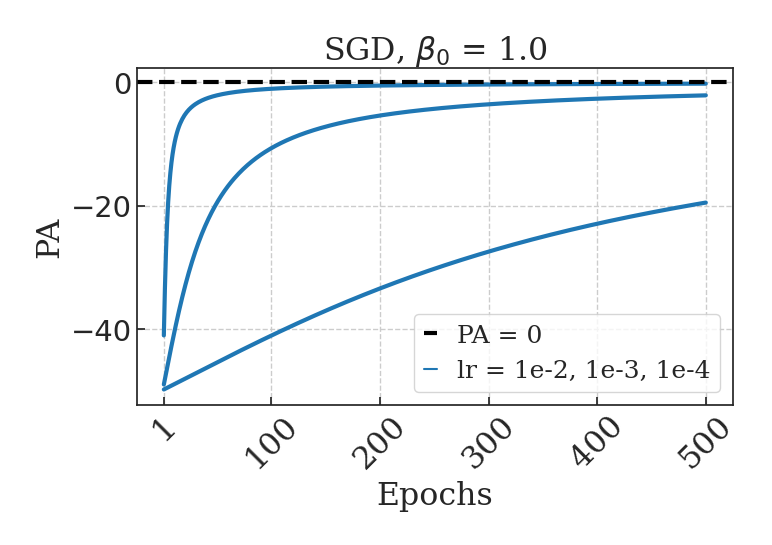
\includegraphics[width=\textwidth]{img/results_discussion/empirical/rob_met=logPA_hue=lr_opt=sgd_beta0=1.0.png}
    \end{subfigure}
    \hfill
    \begin{subfigure}[b]{0.45\textwidth}
        \centering
        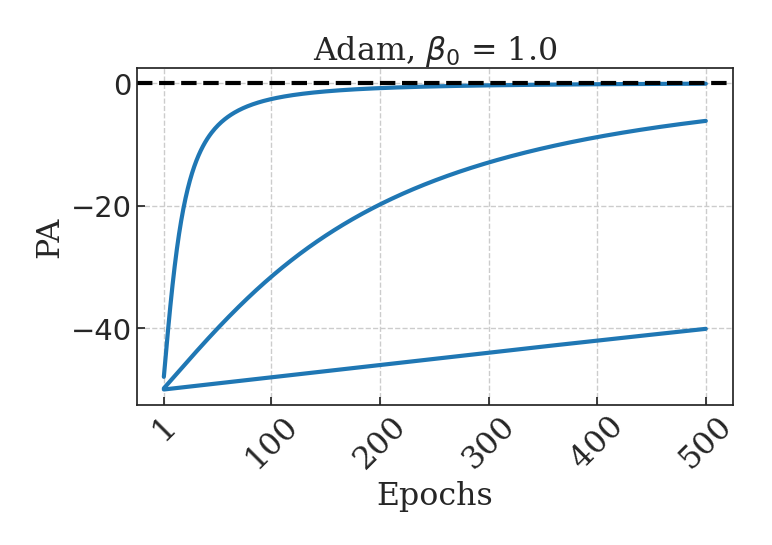
\includegraphics[width=\textwidth]{img/results_discussion/empirical/rob_met=logPA_hue=lr_opt=adam_beta0=1.0.png}
    \end{subfigure}
    \caption{Evolution of the $\beta$ optimization for a robust sample.}
\end{figure}

\begin{figure}[H]
    \centering
    \begin{subfigure}[b]{0.45\textwidth}
        \centering
        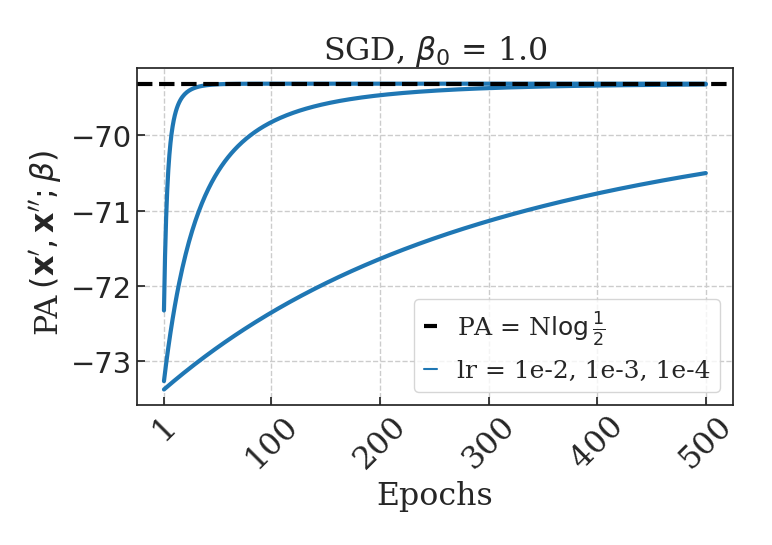
\includegraphics[width=\textwidth]{img/results_discussion/empirical/nonrob_met=logPA_hue=lr_opt=sgd_beta0=1.0.png}
    \end{subfigure}
    \hfill
    \begin{subfigure}[b]{0.45\textwidth}
        \centering
        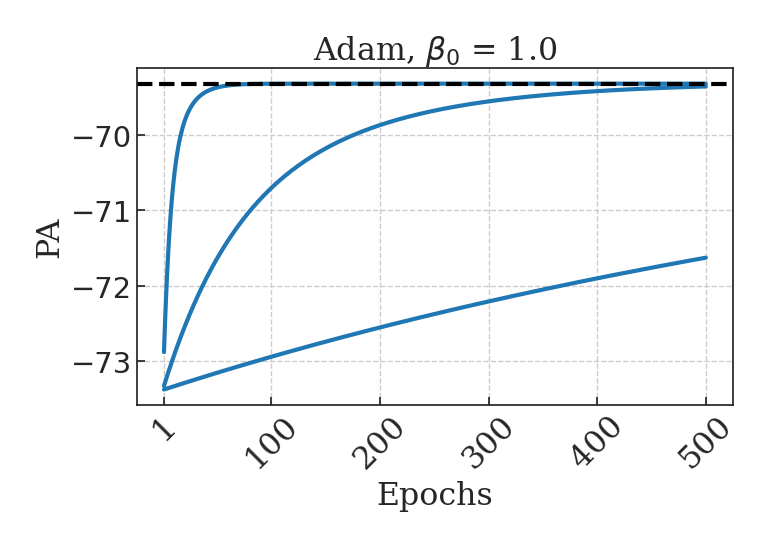
\includegraphics[width=\textwidth]{img/results_discussion/empirical/nonrob_met=logPA_hue=lr_opt=adam_beta0=1.0.png}
    \end{subfigure}
    \caption{Evolution of the $\beta$ optimization for a non-robust sample.}
\end{figure}

The bernoulli sample simulation allows us also to assess the behaviour of the PA
metric under different levels of prediction confidence. For instance, it was shown in
Figure \ref{fig:prediction_confidence} that the value of $\beta^{*}$ is highly informative
of the nature of the model's output probability distribution, and could be an indication of
possible underfitting or overfitting to specific features of the training set, which is highly
valuable in the covariate shift setting.

\begin{figure}[H]
    \centering
    \begin{subfigure}[b]{0.2\textwidth}
        \centering
        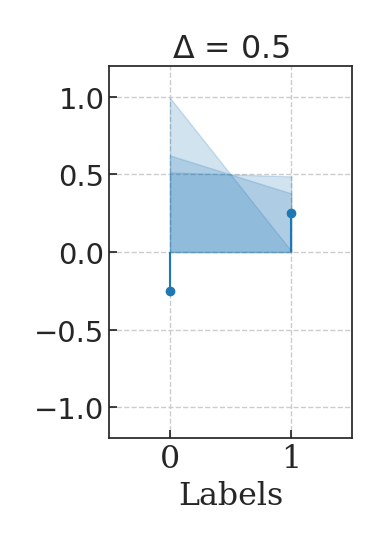
\includegraphics[width=\textwidth]{img/results_discussion/empirical/ldiff=0.5.png}
    \end{subfigure}
    \hfill
    \begin{subfigure}[b]{0.2\textwidth}
        \centering
        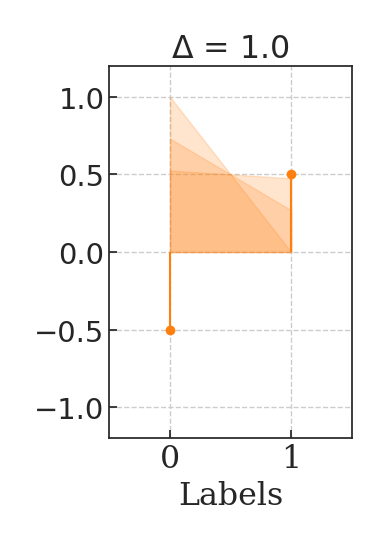
\includegraphics[width=\textwidth]{img/results_discussion/empirical/ldiff=1.0.png}
    \end{subfigure}
    \hfill
    \begin{subfigure}[b]{0.2\textwidth}
        \centering
        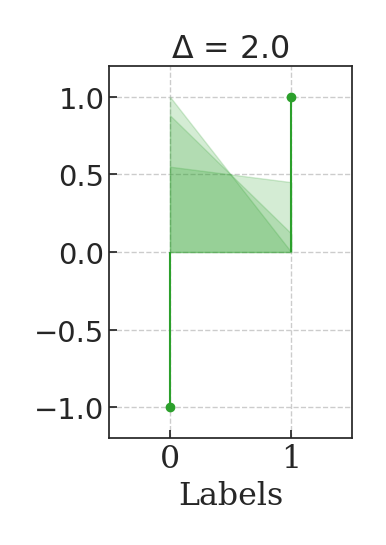
\includegraphics[width=\textwidth]{img/results_discussion/empirical/ldiff=2.0.png}
    \end{subfigure}
    \caption{Logit distributions associated with the behaviour observed in Figure \ref{fig:prediction_confidence}.}
\end{figure}

We see that in the case of a non-robust model, the higher the beta the more pointy is the distribution. Given that 
many samples are completely misaligned, the highest $\beta$ will be zero, which is when the distribution is completely 
flat. The smaller is the difference in the logits, the less pointy is the distribution for $\beta > 0$, which means 
that the overlap will be higher. \\

Finally, we can also check whether the optimization of the kernel is consistent
with results on its concavity and the existence of a unique maximum. The following figures
show that optimization converges for $0 < \beta < M$, with $M$ large enough so that concavity
is less and less defined.

\begin{figure}[H]
    \centering
    \begin{subfigure}[b]{0.45\textwidth}
        \centering
        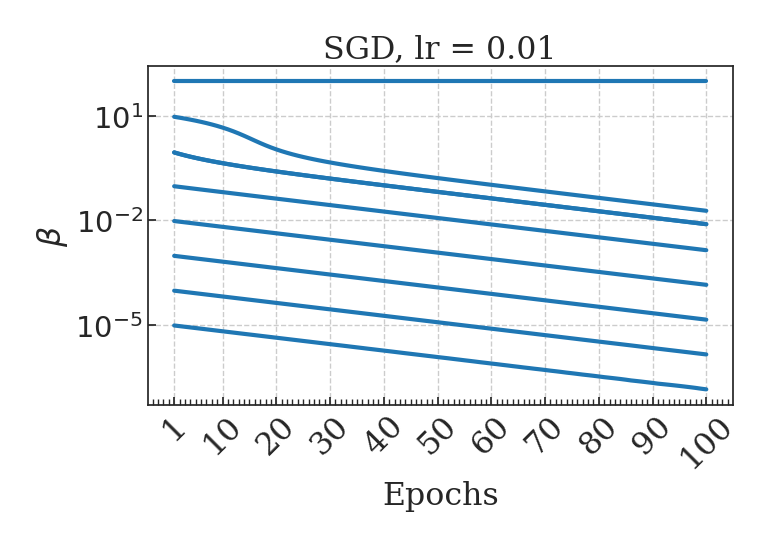
\includegraphics[width=\textwidth]{img/results_discussion/empirical/nonrob_met=betas_hue=beta0_opt=sgd_lr=0.01.png}
    \end{subfigure}
    \hfill
    \begin{subfigure}[b]{0.45\textwidth}
        \centering
        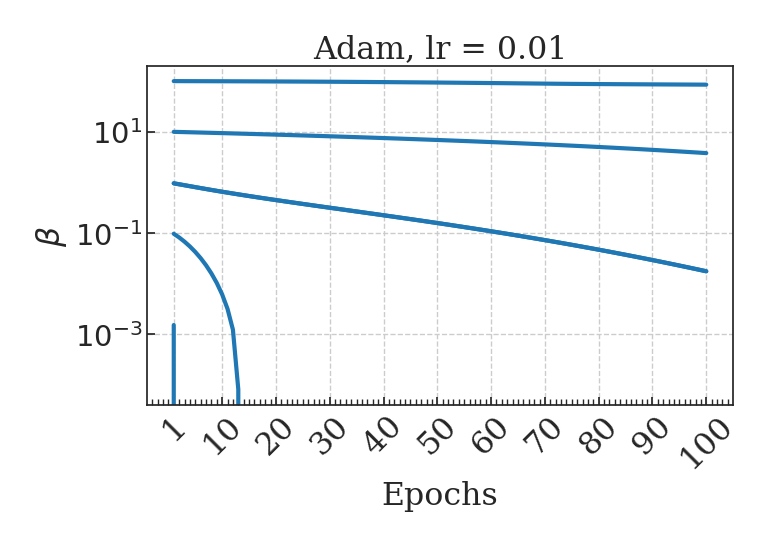
\includegraphics[width=\textwidth]{img/results_discussion/empirical/nonrob_met=betas_hue=beta0_opt=adam_lr=0.01.png}
    \end{subfigure}
    \caption{Evolution of $\beta$ optimization for different initial values for a non-robust classifier.}
\end{figure}

\begin{figure}[H]
    \centering
    \begin{subfigure}[b]{0.45\textwidth}
        \centering
        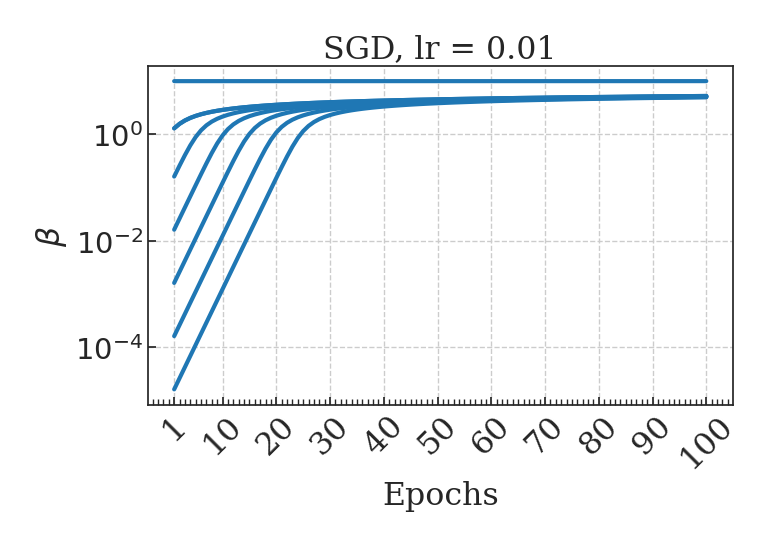
\includegraphics[width=\textwidth]{img/results_discussion/empirical/rob_met=betas_hue=beta0_opt=sgd_lr=0.01.png}
    \end{subfigure}
    \hfill
    \begin{subfigure}[b]{0.45\textwidth}
        \centering
        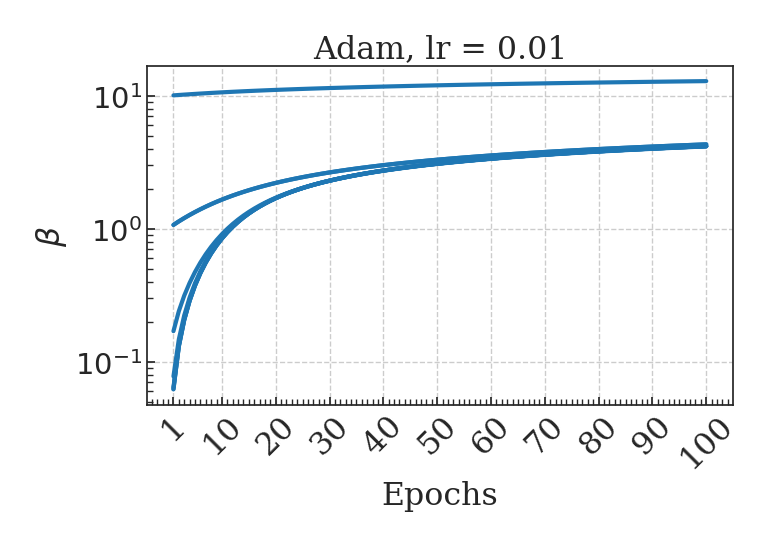
\includegraphics[width=\textwidth]{img/results_discussion/empirical/rob_met=betas_hue=beta0_opt=adam_lr=0.01.png}
    \end{subfigure}
    \caption{Evolution of $\beta$ optimization for different initial values for a robust classifier.}
\end{figure}



\section{Adversarial setting}\label{sec:appendix_results_adversarial}

The first result provided in the adversarial setting is the entropy difference
between initial (i.e. $\beta=1$) and optimal posterior distributions, which is shown
to decrease significantly in robust models, due to the fact that few samples
are misclassified and therefore maximum agreement is achieved with higher
inverse temperature values. Entropy is computed for the average posterior distribution
on correctly classified samples, which represent the largest portion of the dataset.

\begin{figure}[H]
    \centering
    \begin{subfigure}[b]{0.45\textwidth}
        \centering
        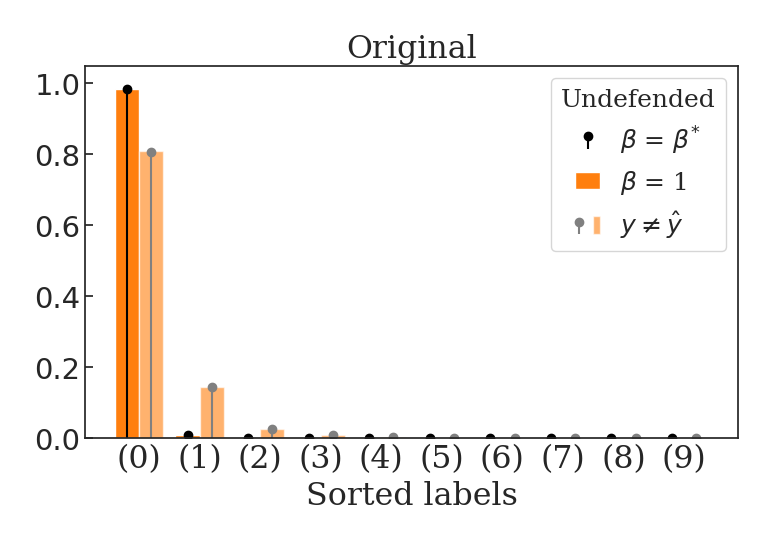
\includegraphics[width=\textwidth]{img/results_discussion/adversarial/Standard_orig_PGD_0.0314.png}
    \end{subfigure}
    \hfill
    \begin{subfigure}[b]{0.45\textwidth}
        \centering
        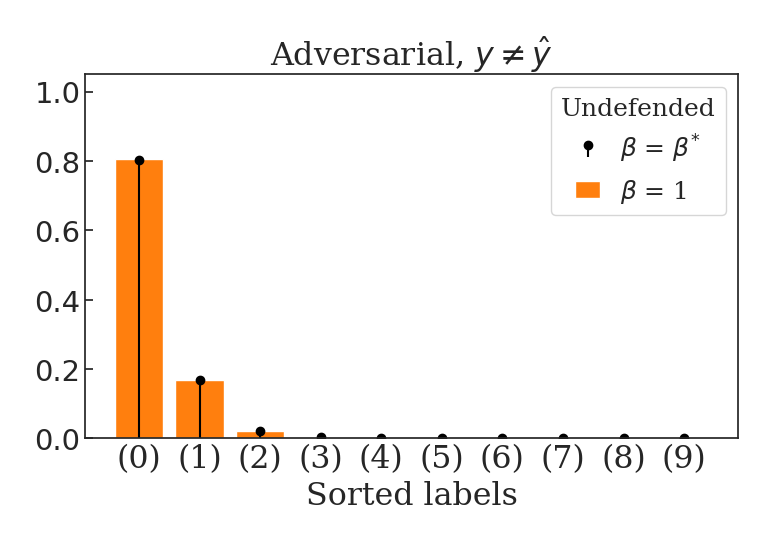
\includegraphics[width=\textwidth]{img/results_discussion/adversarial/Standard_adv_PGD_0.0314.png}
    \end{subfigure}

    \caption{Average $\mathbf{P}(\hat{y}^\prime \mid \mathbf{x}^\prime, \hat{y}^{\prime \prime} = \hat{y}^\prime = y)$,
    $\mathbf{P}(\hat{y}^\prime \mid \mathbf{x}^\prime, \hat{y}^{\prime \prime} = \hat{y}^\prime \neq y)$ and
    $\mathbf{P}(\hat{y}^{\prime \prime} \mid \mathbf{x}^{\prime \prime}, \hat{y}^{\prime \prime} \neq \hat{y}^\prime)$,
    respectively. {\color{tab:orange} \textbf{Undefended}} model under PGD attack, $\ell_\infty$=8/255.}
    \label{fig:pgd_distributions_undefended}
\end{figure}
\begin{figure}[H]
    \centering
    \begin{subfigure}[b]{0.45\textwidth}
        \centering
        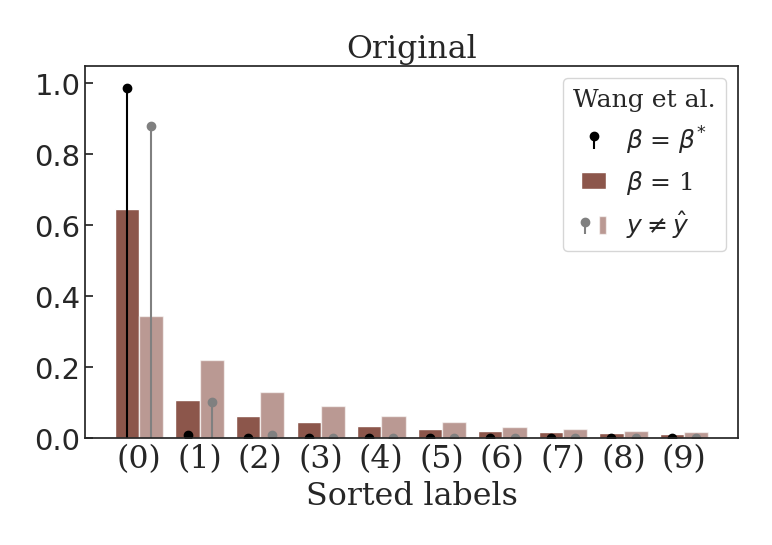
\includegraphics[width=\textwidth]{img/results_discussion/adversarial/Wang2023Better_WRN-28-10_orig_PGD_0.0314.png}
    \end{subfigure}
    \hfill
    \begin{subfigure}[b]{0.45\textwidth}
        \centering
        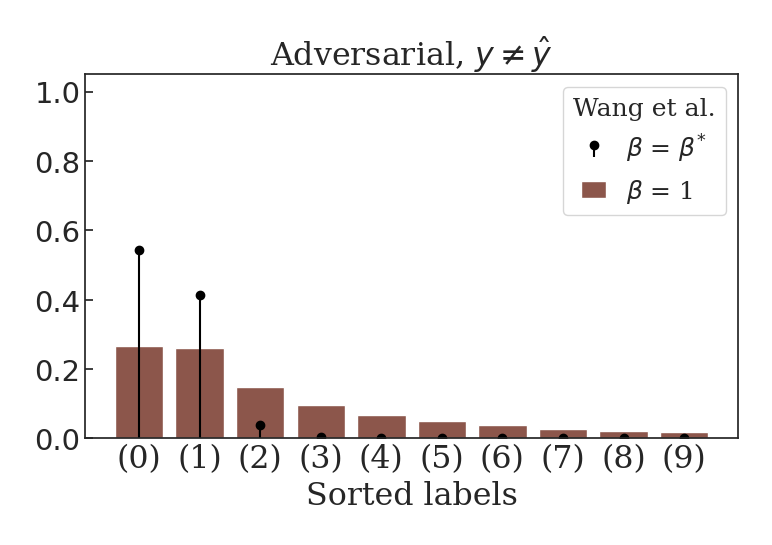
\includegraphics[width=\textwidth]{img/results_discussion/adversarial/Wang2023Better_WRN-28-10_adv_PGD_0.0314.png}
    \end{subfigure}

    \caption{Average $\mathbf{P}(\hat{y}^\prime \mid \mathbf{x}^\prime, \hat{y}^{\prime \prime} = \hat{y}^\prime = y)$,
    $\mathbf{P}(\hat{y}^\prime \mid \mathbf{x}^\prime, \hat{y}^{\prime \prime} = \hat{y}^\prime \neq y)$ and
    $\mathbf{P}(\hat{y}^{\prime \prime} \mid \mathbf{x}^{\prime \prime}, \hat{y}^{\prime \prime} \neq \hat{y}^\prime)$,
    respectively. {\color{tab:brown} \textbf{Wang et al.}} model under PGD attack, $\ell_\infty$=8/255.}
    \label{fig:pgd_distributions_wang2023}
\end{figure}
\begin{figure}[H]
    \centering
    \begin{subfigure}[b]{0.45\textwidth}
        \centering
        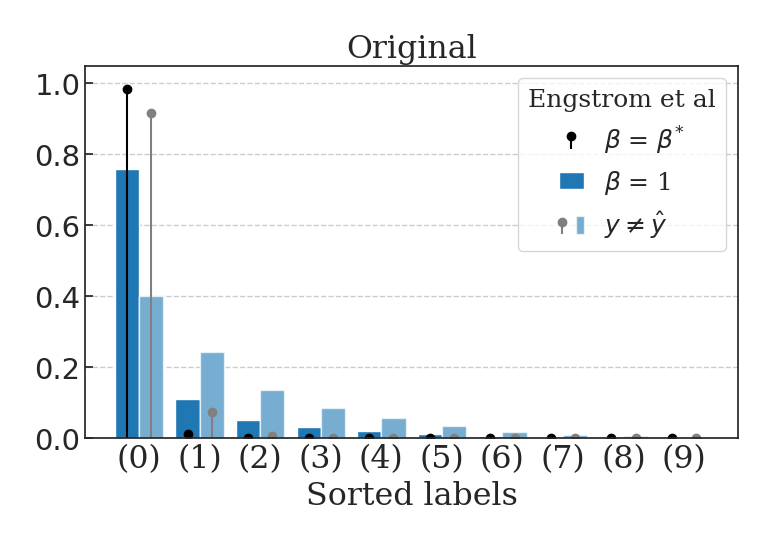
\includegraphics[width=\textwidth]{img/results_discussion/adversarial/Engstrom2019Robustness_orig_PGD_0.0314.png}
    \end{subfigure}
    \hfill
    \begin{subfigure}[b]{0.45\textwidth}
        \centering
        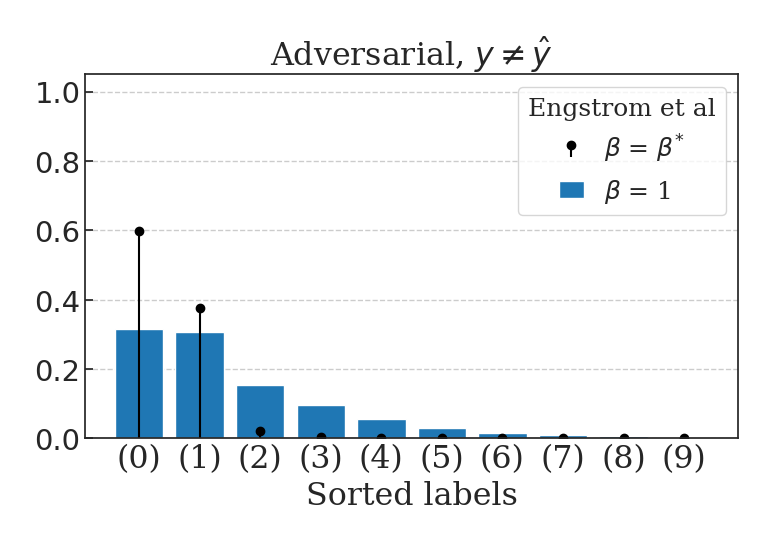
\includegraphics[width=\textwidth]{img/results_discussion/adversarial/Engstrom2019Robustness_adv_PGD_0.0314.png}
    \end{subfigure}

    \caption{Average $\mathbf{P}(\hat{y}^\prime \mid \mathbf{x}^\prime, \hat{y}^{\prime \prime} = \hat{y}^\prime = y)$,
    $\mathbf{P}(\hat{y}^\prime \mid \mathbf{x}^\prime, \hat{y}^{\prime \prime} = \hat{y}^\prime \neq y)$ and
    $\mathbf{P}(\hat{y}^{\prime \prime} \mid \mathbf{x}^{\prime \prime}, \hat{y}^{\prime \prime} \neq \hat{y}^\prime)$,
    respectively. {\color{tab:blue} \textbf{Engstrom et al.}} model under PGD attack, $\ell_\infty$=8/255.}
    \label{fig:pgd_distributions_engstrom}
\end{figure}
\begin{figure}[H]
    \centering
    \begin{subfigure}[b]{0.45\textwidth}
        \centering
        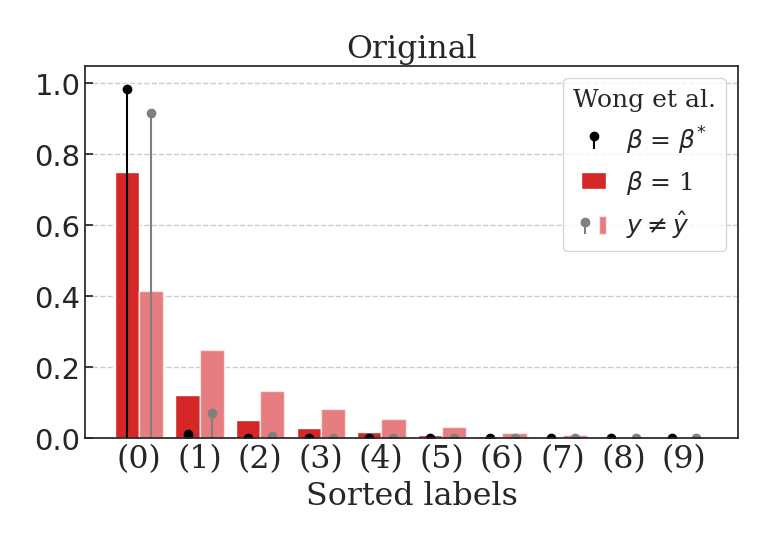
\includegraphics[width=\textwidth]{img/results_discussion/adversarial/Wong2020Fast_orig_PGD_0.0314.png}
    \end{subfigure}
    \hfill
    \begin{subfigure}[b]{0.45\textwidth}
        \centering
        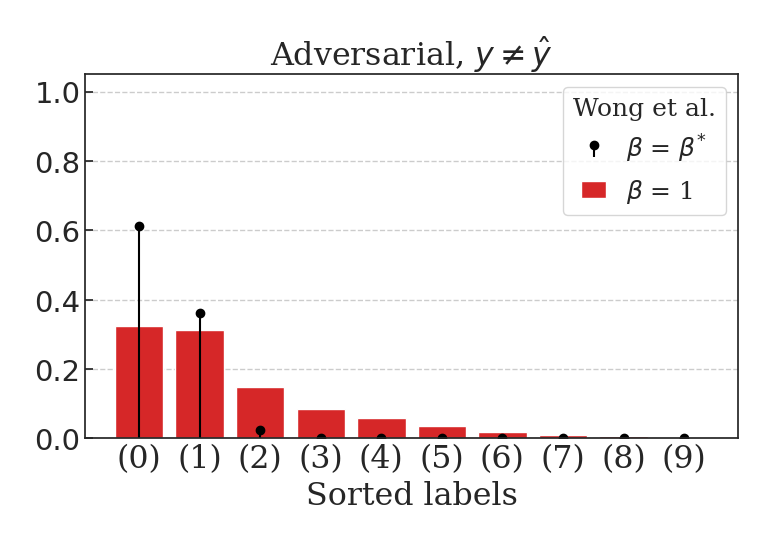
\includegraphics[width=\textwidth]{img/results_discussion/adversarial/Wong2020Fast_adv_PGD_0.0314.png}
    \end{subfigure}

    \caption{Average $\mathbf{P}(\hat{y}^\prime \mid \mathbf{x}^\prime, \hat{y}^{\prime \prime} = \hat{y}^\prime = y)$,
    $\mathbf{P}(\hat{y}^\prime \mid \mathbf{x}^\prime, \hat{y}^{\prime \prime} = \hat{y}^\prime \neq y)$ and
    $\mathbf{P}(\hat{y}^{\prime \prime} \mid \mathbf{x}^{\prime \prime}, \hat{y}^{\prime \prime} \neq \hat{y}^\prime)$,
    respectively. {\color{tab:red} \textbf{Wong et al.}} model under PGD attack, $\ell_\infty$=8/255.}
    \label{fig:pgd_distributions_wong2020}
\end{figure}
\begin{figure}[H]
    \centering
    \begin{subfigure}[b]{0.45\textwidth}
        \centering
        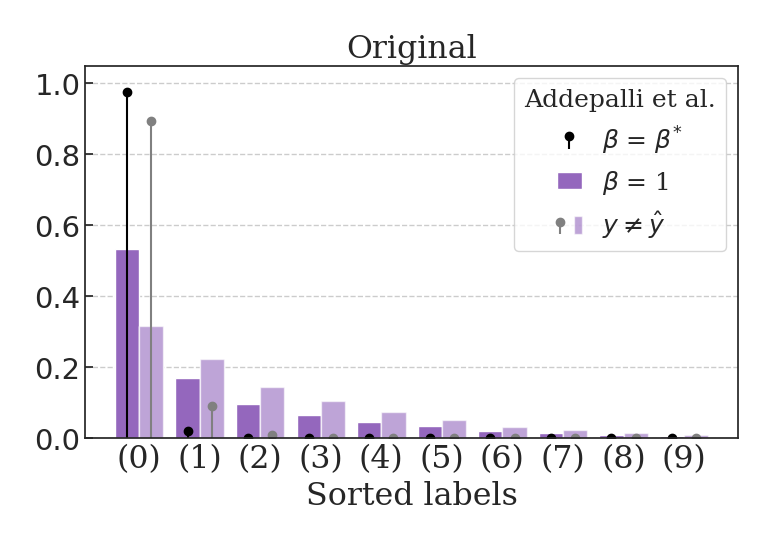
\includegraphics[width=\textwidth]{img/results_discussion/adversarial/Addepalli2021Towards_RN18_orig_PGD_0.0314.png}
    \end{subfigure}
    \hfill
    \begin{subfigure}[b]{0.45\textwidth}
        \centering
        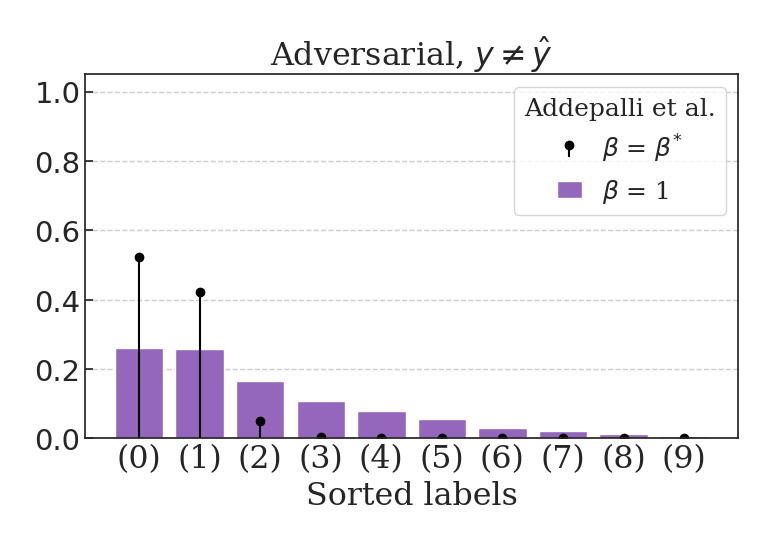
\includegraphics[width=\textwidth]{img/results_discussion/adversarial/Addepalli2021Towards_RN18_adv_PGD_0.0314.png}
    \end{subfigure}

    \caption{Average $\mathbf{P}(\hat{y}^\prime \mid \mathbf{x}^\prime, \hat{y}^{\prime \prime} = \hat{y}^\prime = y)$,
    $\mathbf{P}(\hat{y}^\prime \mid \mathbf{x}^\prime, \hat{y}^{\prime \prime} = \hat{y}^\prime \neq y)$ and
    $\mathbf{P}(\hat{y}^{\prime \prime} \mid \mathbf{x}^{\prime \prime}, \hat{y}^{\prime \prime} \neq \hat{y}^\prime)$,
    respectively. {\color{tab:purple} \textbf{Addepalli et al.}} model under PGD attack, $\ell_\infty$=8/255.}
    \label{fig:pgd_distributions_addepalli2021}
\end{figure}
\begin{figure}[H]
    \centering
    \begin{subfigure}[b]{0.45\textwidth}
        \centering
        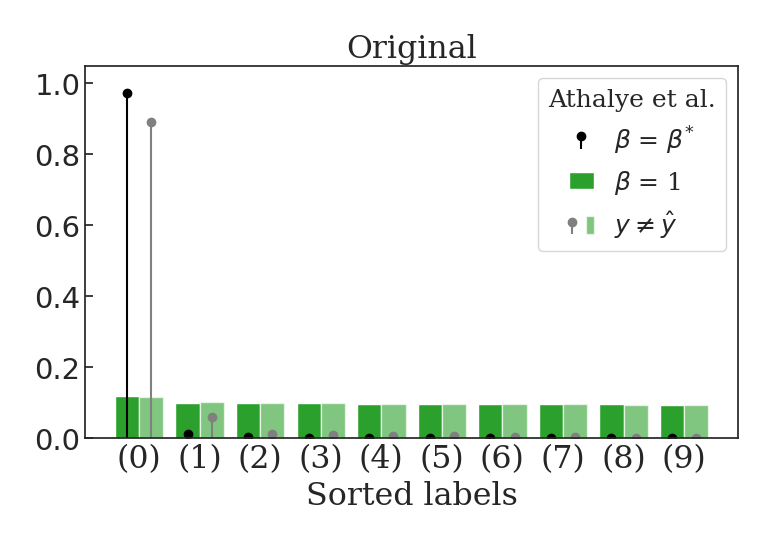
\includegraphics[width=\textwidth]{img/results_discussion/adversarial/BPDA_orig_PGD_0.0314.png}
    \end{subfigure}
    \hfill
    \begin{subfigure}[b]{0.45\textwidth}
        \centering
        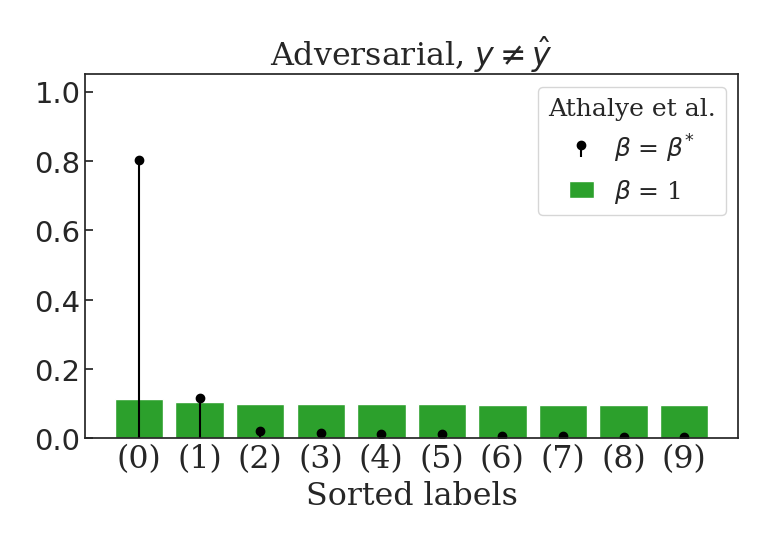
\includegraphics[width=\textwidth]{img/results_discussion/adversarial/BPDA_adv_PGD_0.0314.png}
    \end{subfigure}

    \caption{Average $\mathbf{P}(\hat{y}^\prime \mid \mathbf{x}^\prime, \hat{y}^{\prime \prime} = \hat{y}^\prime = y)$,
    $\mathbf{P}(\hat{y}^\prime \mid \mathbf{x}^\prime, \hat{y}^{\prime \prime} = \hat{y}^\prime \neq y)$ and
    $\mathbf{P}(\hat{y}^{\prime \prime} \mid \mathbf{x}^{\prime \prime}, \hat{y}^{\prime \prime} \neq \hat{y}^\prime)$,
    respectively. {\color{tab:green} \textbf{Athalye et al.}} model under PGD attack, $\ell_\infty$=8/255.}
    \label{fig:pgd_distributions_bpda}
\end{figure}

One of the claims made about PA is that its discriminative power is superior to that
of AFR, because its value is not so much driven by the sampling randomness associated
to a specific experiment (i.e. dataset), and therefore provides a more reliable
assessment of the robustness capabilities of the model. We can observe that AFR(P),
which is by definition the baseline measure of robustness in the adversarial setting,
is way less discriminative and fluctuates its value significantly over different
presence of adversarial samples.

\begin{figure}[H]
    \centering
    \begin{subfigure}[b]{0.45\textwidth}
        \centering
        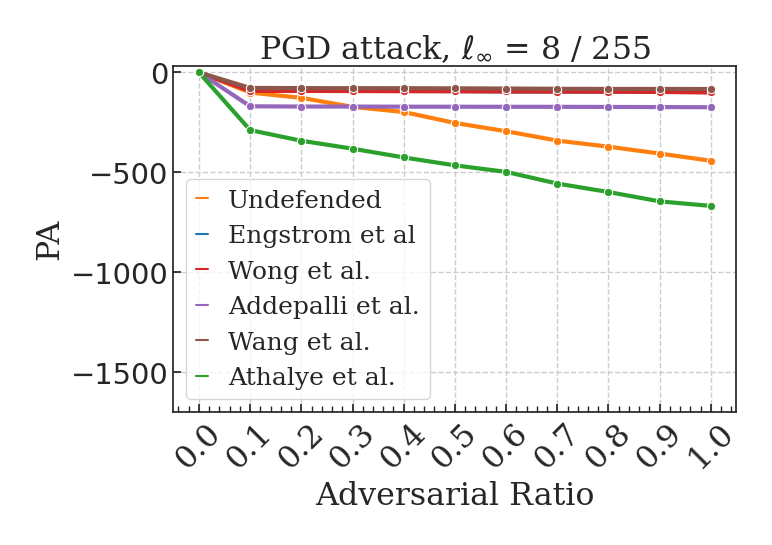
\includegraphics[width=\textwidth]{img/results_discussion/adversarial/PGD_0.0314_logPA_linear.png}
    \end{subfigure}
    \begin{subfigure}[b]{0.45\textwidth}
        \centering
        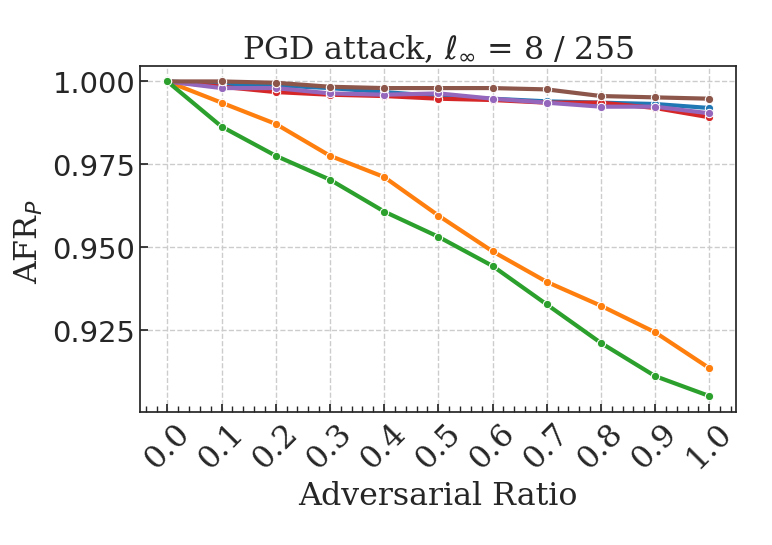
\includegraphics[width=\textwidth]{img/results_discussion/adversarial/PGD_0.0314_AFR_pred.png}
    \end{subfigure}

    \vspace{1em}

    \begin{subfigure}[b]{0.45\textwidth}
        \centering
        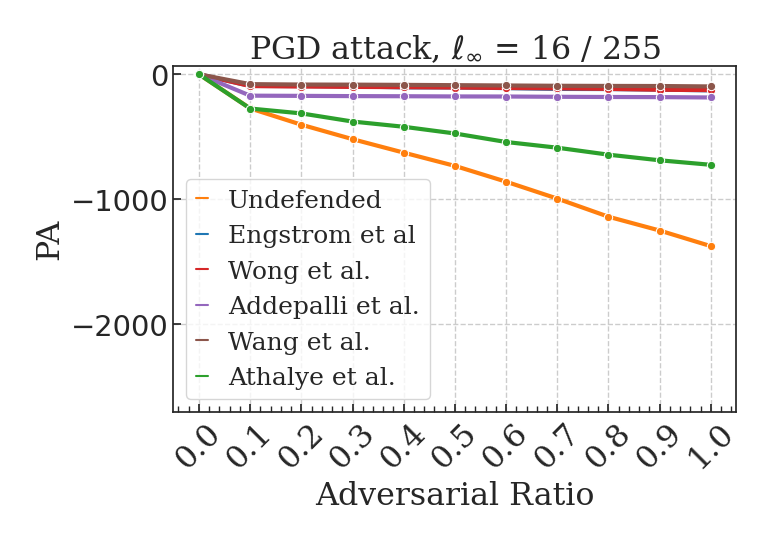
\includegraphics[width=\textwidth]{img/results_discussion/adversarial/PGD_0.0627_logPA_linear.png}
    \end{subfigure}
    \begin{subfigure}[b]{0.45\textwidth}
        \centering
        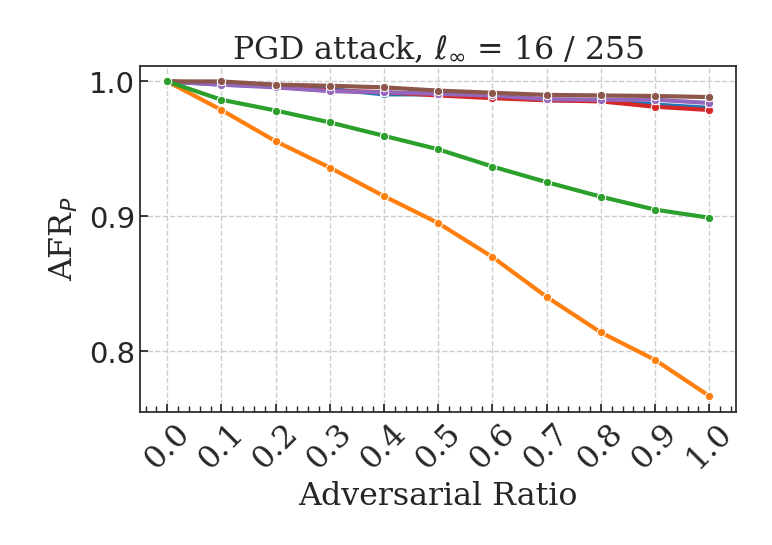
\includegraphics[width=\textwidth]{img/results_discussion/adversarial/PGD_0.0627_AFR_pred.png}
    \end{subfigure}

    \vspace{1em}

    \begin{subfigure}[b]{0.45\textwidth}
        \centering
        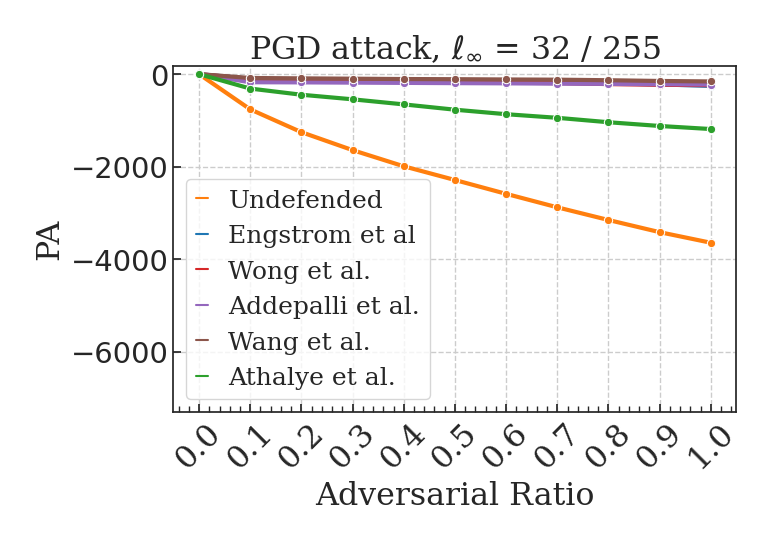
\includegraphics[width=\textwidth]{img/results_discussion/adversarial/PGD_0.1255_logPA_linear.png}
    \end{subfigure}
    \begin{subfigure}[b]{0.45\textwidth}
        \centering
        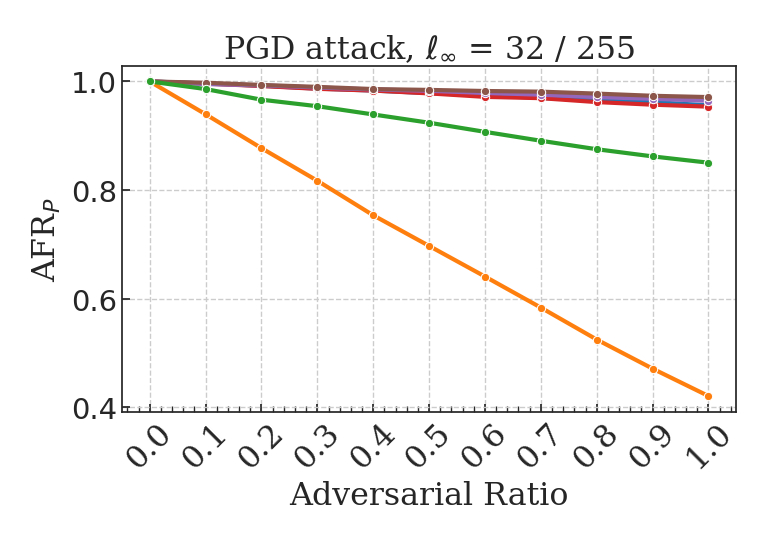
\includegraphics[width=\textwidth]{img/results_discussion/adversarial/PGD_0.1255_AFR_pred.png}
    \end{subfigure}

    \caption{PA and AFR(P) variation under increasing adversarial ratio at different
    perturbation norm bounds. The undefended net and several RobustBench
    robust models are considered against a 1000 step PGD attack.}
    \label{fig:appendix_adversarial_afrpred_pgd}
\end{figure}

\begin{figure}[H]
    \centering
    \begin{subfigure}[b]{0.45\textwidth}
        \centering
        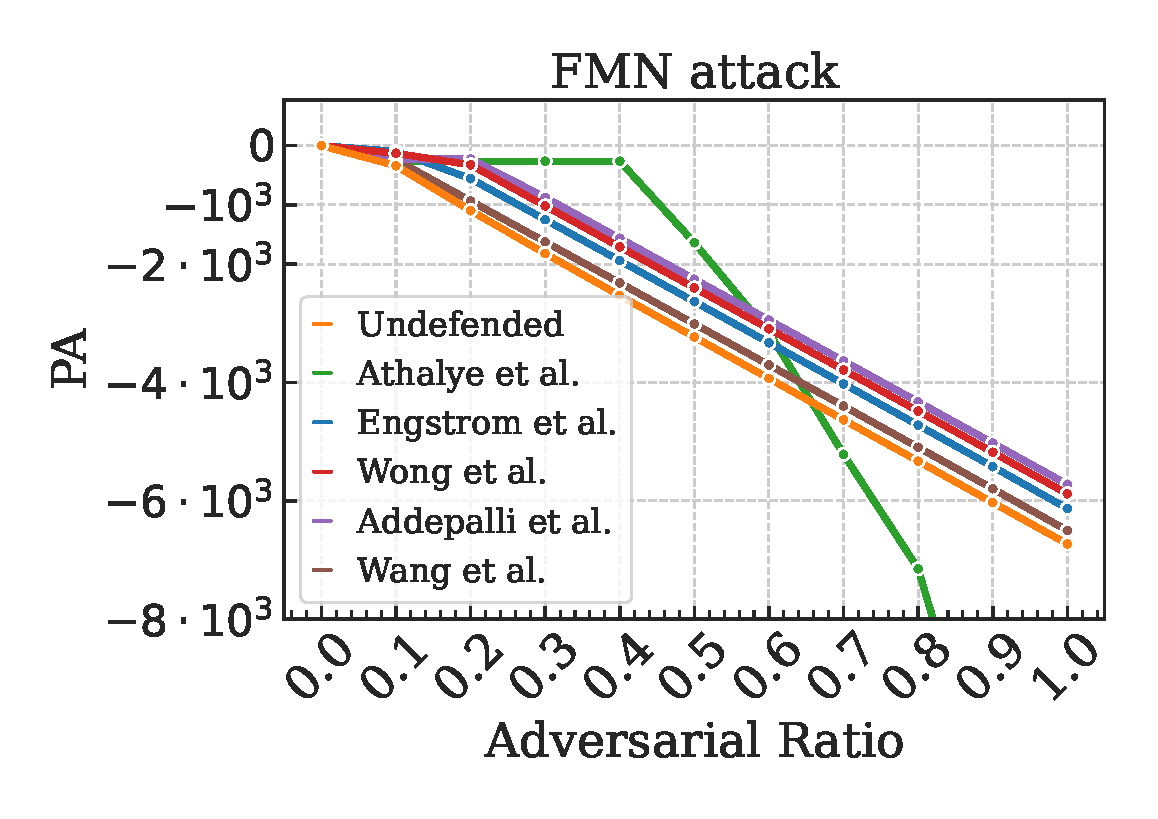
\includegraphics[width=\textwidth]{img/results_discussion/adversarial/FMN.pdf}
    \end{subfigure}
    \begin{subfigure}[b]{0.45\textwidth}
        \centering
        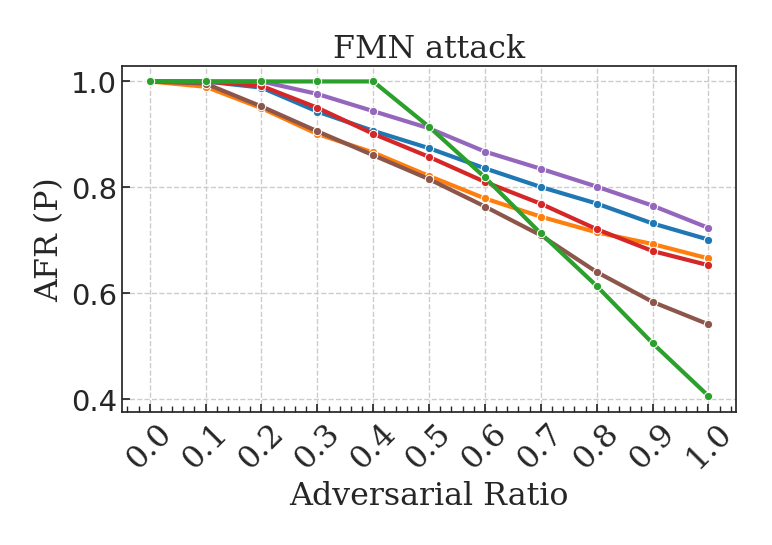
\includegraphics[width=\textwidth]{img/results_discussion/adversarial/FMN_1000_AFR_pred.png}
    \end{subfigure}

    \caption{PA and AFR(P) variation under increasing adversarial ratio. T
    he undefended net and several RobustBench robust models are considered 
    against a 1000 step FMN attack.}
    \label{fig:appendix_adversarial_afrpred_fmn}
\end{figure}

Another claim that was made is the fact that optimal posterior distributions are
assumed to be highly peaked at the predicted class. This assumption allows us to
break down the PA robustness score into a sum of terms that represent specific
contributions to the robustness of the model, and that can be approximated
analytically.

\begin{theorem}[Approximated PA in the adversarial setting]
    The assumption of a peaked gibbs posterior allows approximate the maximum PA value as follows:

    $$
        \operatorname{PA} \approx N\tau \rho \log \left( 1 - 2\delta_{\text{ERR}} \right) + N(1- \tau) \rho \log \left( 1 - 2\delta_{\text{MIS}} \right)  + N\tau (1 - \rho) \log \delta_{\text{ADV}},
    $$
\end{theorem}
\begin{figure}[H]
    \centering
    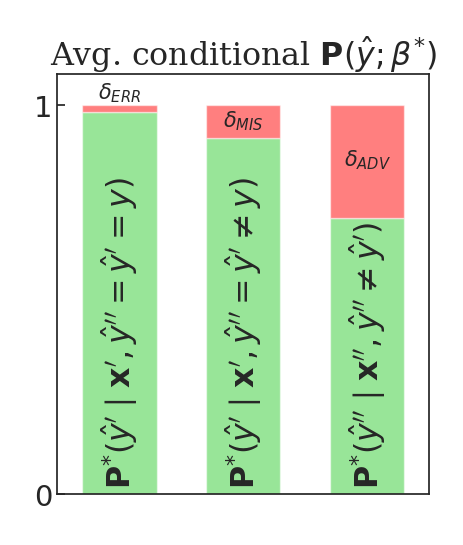
\includegraphics[width=0.4\textwidth]{img/results_discussion/adversarial/demonstration.png}
    \caption{Illustrative representation of the terms and posterior values constrained
    considered for the PA approximation.
    }
    \label{fig:appendix_adv_illustration}
\end{figure}
\begin{proof}
    Let $\hat{y}^\prime$ and $\hat{y}^{\prime \prime}$ be the predicted class for an arbitrary 
    original and an adversarial samples, respectively, and $y_{\text{true}}$ the true class. The first and second
    most likely labels for a sample are obtained as:

    $$
    \begin{aligned}
        \hat{y}_{\text{first}} &= \arg \max_{\mathcal{Y}} \mathbf{P}(y \mid \bm{x}) = \hat{y} \\
        \hat{y}_{\text{next}} &= \arg \max_{\mathcal{Y} \setminus \{ \hat{y} \} } \mathbf{P}(y \mid \bm{x})
    \end{aligned}
    $$

    Let $\mathbf{P}^{*}$ be the optimal posterior distribution over the classes for a
    specific sample; that is, the gibbs distribution with inverse temperature $\beta^{*}$. Following the PA kernel
    expression, the contribution of each pair of samples can be approximated as

    $$
    \Xi = \log \left\{ \sum_{y \in \mathcal{Y}} \mathbf{P}^{*}(y \mid \bm{x}^\prime) \mathbf{P}^{*}(y \mid \bm{x}^{\prime \prime}) \right\}
    \approx \log \left\{ \mathbf{P}^{*}(\hat{y}^\prime \mid \bm{x}^\prime) \mathbf{P}^{*}(\hat{y}^{\prime \prime} \mid \bm{x}^{\prime \prime}) + \mathbf{P}^{*}(\hat{y}_{\text{next}}^\prime \mid \bm{x}^\prime) \mathbf{P}^{*}(\hat{y}_{\text{next}}^{\prime \prime} \mid \bm{x}^{\prime \prime})\right\}.
    $$
    
    Let $\mathfrak{f}$ be the fraction of samples that contribute to the PA value in a specific way for a given
    adversarial ratio, so that $N \mathfrak{f}$ is the number of contributing terms. To avoid notation 
    clutter, we will define:

    $$
    \begin{aligned}
        &\tau = \operatorname{ACC}(\bm{\hat{y}^\prime}, \bm{y_{\text{true}}}) = \operatorname{AFR (T)} \bigg|_{\operatorname{AR} = 0.0} \\
        &\rho = \operatorname{AFR (P)}\bigg|_{\operatorname{AR}}
    \end{aligned}
    $$
    
    Given that optimal posteriors
    are expected to be peaked, these contributions can be approximated for three relevant cases.

    \begin{description}
        \item[Case] $y_{\text{true}} = \hat{y}^{\prime \prime} = \hat{y}^{\prime} = \hat{y}$\textbf{.} Clearly 
        $\mathfrak{f} = \tau \rho$. Then
        $$
        \begin{aligned}
            & \mathbf{P}^{*}(\hat{y} \mid \bm{x}^\prime) \approx \mathbf{P}^{*}(\hat{y} \mid \bm{x}^{\prime \prime}) = 1 - \delta_{\text{ERR}}, \\
            & \mathbf{P}^{*}(\hat{y}_{\text{next}}^{\prime}  \mid \bm{x}^\prime) \approx \mathbf{P}^{*}(\hat{y}_{\text{next}}^{\prime \prime}  \mid \bm{x}^{\prime \prime}) \approx \delta_{\text{ERR}},
        \end{aligned}
        $$
        which yields
        $$
        \Xi_{\text{ERR}}^i \approx \log \left\{ \left(1 - \delta_{\text{ERR}} \right)^2 +  \delta_{\text{ERR}}^ 2 \right\} \approx \log \left( 1 - 2\delta_{\text{ERR}} \right) ,
        $$
        where $\delta_{\text{ERR}}$ represents the lack of confidence when successfully predicting original samples.
        
        \item[Case]$y_{\text{true}} \neq \hat{y}^{\prime \prime} = \hat{y}^{\prime} = \hat{y}$\textbf{.} Clearly $\mathfrak{f} \approx (1 - \tau)\rho$. Then
        $$
        \begin{aligned}
            & \mathbf{P}^{*}(\hat{y} \mid \bm{x}^\prime) \approx \mathbf{P}^{*}(\hat{y} \mid \bm{x}^{\prime \prime}) = 1 - \delta_{\text{MIS}}, \\
            & \mathbf{P}^{*}(\hat{y}_{\text{next}}^{\prime}  \mid \bm{x}^\prime) \approx \mathbf{P}^{*}(\hat{y}_{\text{next}}^{\prime \prime}  \mid \bm{x}^{\prime \prime}) \approx \delta_{\text{MIS}},
        \end{aligned}
        $$
        which yields
        $$
        \Xi_{\text{MIS}}^i \approx \log \left\{ \left(1 - \delta_{\text{MIS}} \right)^2 +  \delta_{\text{MIS}}^ 2 \right\} \approx \log \left( 1 - 2\delta_{\text{MIS}} \right) ,
        $$
        where $\delta_{\text{MIS}}$ represents the missing prediction confidence on misclassified original samples.

        \item[Case]$y_{\text{true}} = \hat{y}^{\prime \prime} \neq \hat{y}^{\prime} = \hat{y}$\textbf{.} Clearly 
        $\mathfrak{f} = \tau (1-\rho)$. Then
        
        $$
        \begin{aligned}
            & \mathbf{P}^{*}(\hat{y}^\prime \mid \bm{x}^\prime) = 1 - \delta_{\text{ERR}},  \\
            & \mathbf{P}^{*}(\hat{y}^{\prime \prime} \mid \bm{x}^\prime) \approx \delta_{\text{ERR}}; \\
            & \mathbf{P}^{*}(\hat{y}^{\prime \prime} \mid \bm{x}^{\prime \prime}) = 1 - \delta_{\text{ADV}}, \\
            & \mathbf{P}^{*}(\hat{y}^{\prime} \mid \bm{x}^{\prime \prime}) \approx \delta_{\text{ADV}},
        \end{aligned}
        $$

        which yields

        $$
        \Xi_{\text{ADV}}^i \approx \log \left\{ \left(1 - \delta_{\text{ERR}} \right) \delta_{\text{ADV}} + \delta_{\text{ERR}} \left(1 - \delta_{\text{ADV}} \right) \right\} \approx \log \delta_{\text{ADV}},
        $$
        given that $\delta_{\text{ERR}} \approx - 2 \delta_{\text{ERR}} \delta_{\text{ADV}}$. $\delta_{\text{ADV}}$ represents the missing confidence in 
        the prediction of a misleading adversarial sample.
    \end{description}

    The approximated PA value amounts to the sum of all contributions.
\end{proof}

The previous expression has been validated empirically with both an FMN attack
and an $\ell_{\infty}$=8/255 PGD attack computed on the CIFAR10 data.

\begin{figure}[H]
    \centering
    \begin{subfigure}[b]{0.45\textwidth}
        \centering
        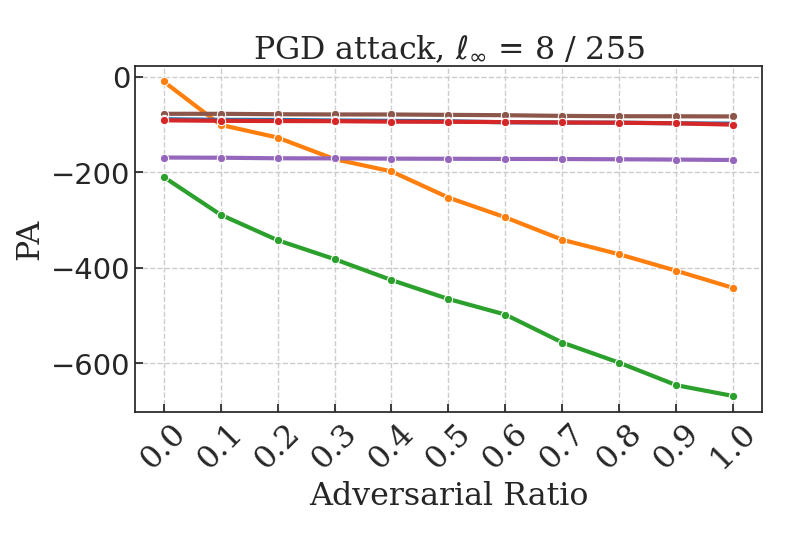
\includegraphics[width=\textwidth]{img/results_discussion/adversarial/pgd_pa_approx.png}
    \end{subfigure}
    \begin{subfigure}[b]{0.45\textwidth}
        \centering
        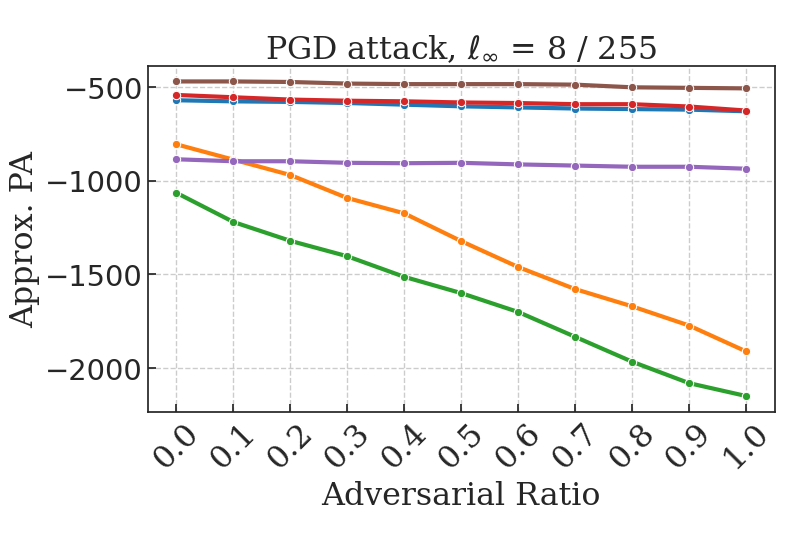
\includegraphics[width=\textwidth]{img/results_discussion/adversarial/pgd_pa_approx_approx.png}
    \end{subfigure}

    \caption{True and approximated PA values under increasing adversarial ratio for
    a PGD attack with $\ell_\infty$=8/255.}
    \label{fig:appendix_adversarial_approx_pa_pgd}
\end{figure}

\begin{figure}[H]
    \centering
    \begin{subfigure}[b]{0.45\textwidth}
        \centering
        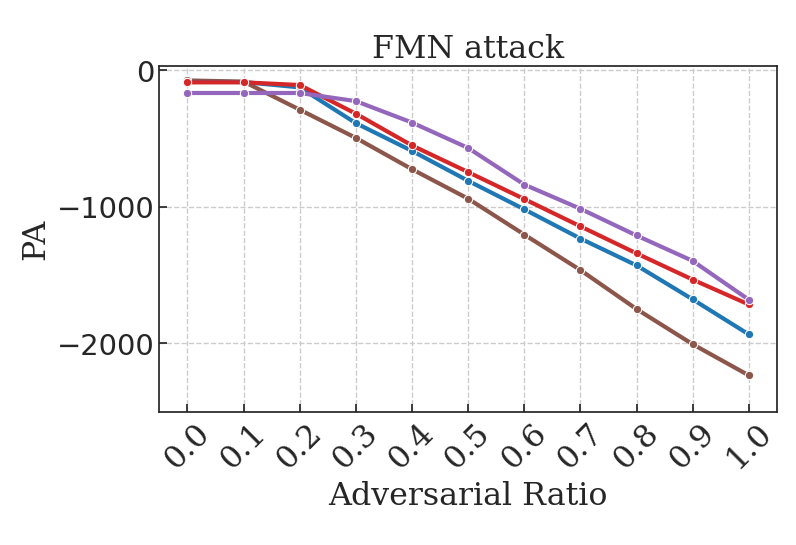
\includegraphics[width=\textwidth]{img/results_discussion/adversarial/fmn_pa_approx.png}
    \end{subfigure}
    \begin{subfigure}[b]{0.45\textwidth}
        \centering
        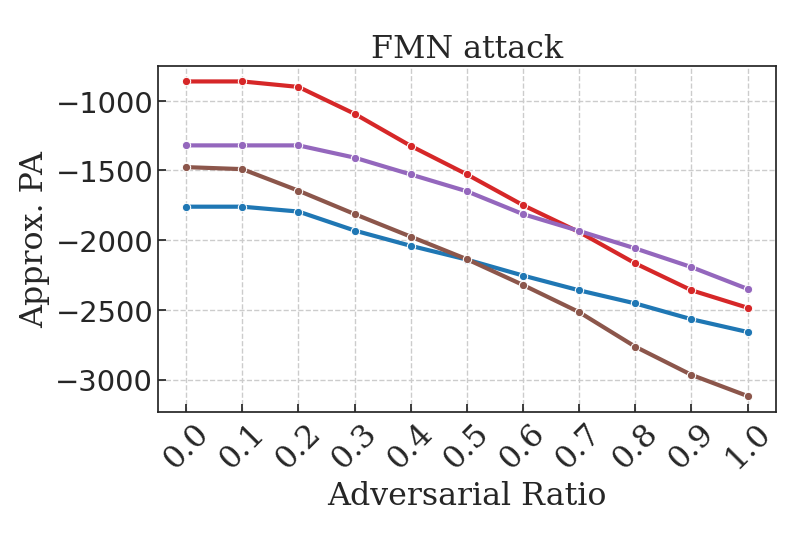
\includegraphics[width=\textwidth]{img/results_discussion/adversarial/fmn_pa_approx_approx.png}
    \end{subfigure}

    \caption{True and approximated PA values under increasing adversarial ratio for
    a FMN attack.}
    \label{fig:appendix_adversarial_approx_pa_fmn}
\end{figure}

Results obtained for for this section illustrate the higher effectiveness of FMN with respect
to PGD attacks in the adversarial dataset. Further insight into the response of the models in each case
can be obtained by comparing the average posterior distributions on original samples, originally
misclassified samples and adversarial samples.

\begin{figure}[H]
    \centering
    \begin{subfigure}[b]{0.3\textwidth}
        \centering
        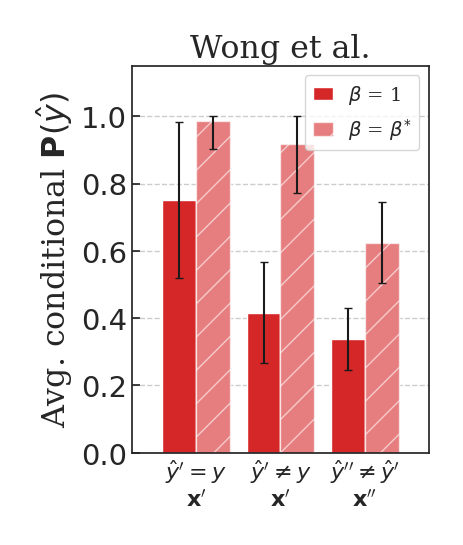
\includegraphics[width=\textwidth]{img/results_discussion/adversarial/Wong2020Fast_short_PGD_0.0314_0.png}
    \end{subfigure}
    \begin{subfigure}[b]{0.3\textwidth}
        \centering
        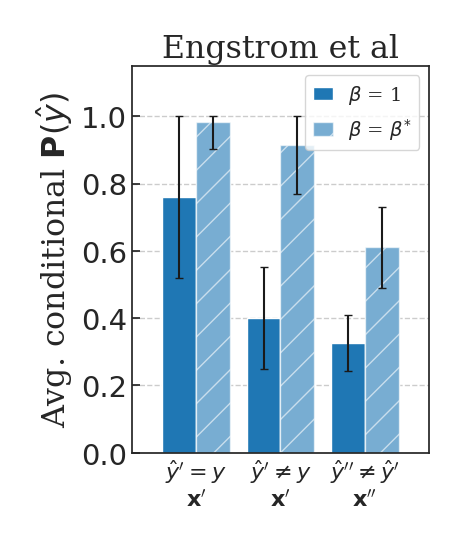
\includegraphics[width=\textwidth]{img/results_discussion/adversarial/Engstrom2019Robustness_short_PGD_0.0314_0.png}
    \end{subfigure}
    \begin{subfigure}[b]{0.3\textwidth}
        \centering
        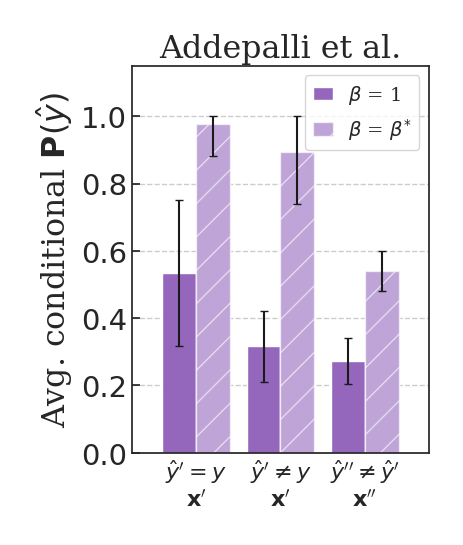
\includegraphics[width=\textwidth]{img/results_discussion/adversarial/Addepalli2021Towards_RN18_short_PGD_0.0314_0.png}
    \end{subfigure}
   
    \caption{Average posterior probability of the predicted class for 
    correctly classified original samples, misclassified original samples, and 
    misleading adversarial samples, respectively. Results have been obtained through a PGD attack with 
    $\ell_\infty$=8/255 and sorted by increasing $\beta^{*}$.}
    \label{fig:appendix_adversarial_distribution_pgd}
\end{figure}

\begin{figure}[H]
    \centering
    \begin{subfigure}[b]{0.3\textwidth}
        \centering
        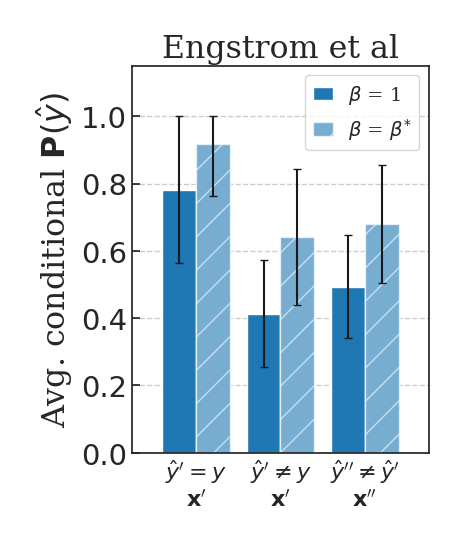
\includegraphics[width=\textwidth]{img/results_discussion/adversarial/Engstrom2019Robustness_short_FMN_0.png}
    \end{subfigure}
    \begin{subfigure}[b]{0.3\textwidth}
        \centering
        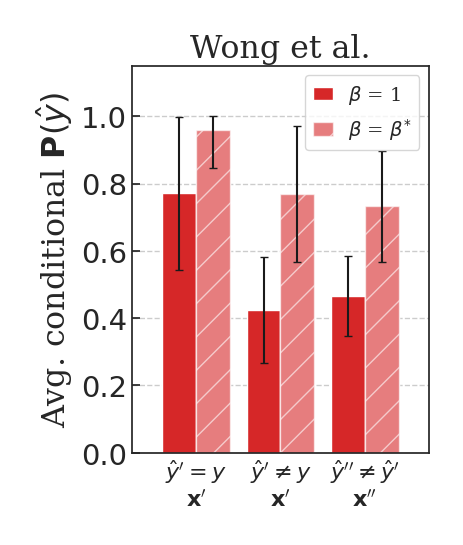
\includegraphics[width=\textwidth]{img/results_discussion/adversarial/Wong2020Fast_short_FMN_0.png}
    \end{subfigure}
    \begin{subfigure}[b]{0.3\textwidth}
        \centering
        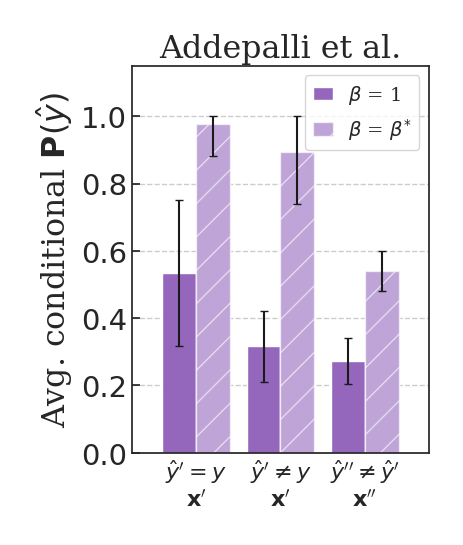
\includegraphics[width=\textwidth]{img/results_discussion/adversarial/Addepalli2021Towards_RN18_short_PGD_0.0314_0.png}
    \end{subfigure}
   
    \caption{Average posterior probability of the predicted class for 
    correctly classified original samples, misclassified original samples, and 
    misleading adversarial samples, respectively. Results have been obtained through a FMN attack 
    and sorted by increasing $\beta^{*}$.}
    \label{fig:appendix_adversarial_distribution_fmn}
\end{figure}


 \cleardoublepage

